\documentclass[conference]{IEEEtran}
\IEEEoverridecommandlockouts
% \IEEEpubid{\makebox[\textwidth]{\textbf{978-1-6654-4146-9/21/\$31.00~\copyright2021 IEEE} \hfill}}

\usepackage{cite}
\usepackage{amsmath,amssymb,amsfonts}
\usepackage{graphicx}
\usepackage{svg}
\usepackage{textcomp}
\usepackage{xcolor}

% folder gambar
\graphicspath{{./figures/}}


\def\BibTeX{{\rm B\kern-.05em{\sc i\kern-.025em b}\kern-.08em
    T\kern-.1667em\lower.7ex\hbox{E}\kern-.125emX}}

% change index term to keywords
\renewcommand\IEEEkeywordsname{Keywords}

\begin{document}

\title{GPS-based Vehicle Tracking and Theft Detection Systems using Google Cloud IoT Core \& Firebase}

\author{
\IEEEauthorblockN{Puji Valen Crisgar\textsuperscript{1}, Patrick Ryan Wijaya\textsuperscript{2}, Marcell D. F. Pakpahan\textsuperscript{3},\\ Eniman Yunus Syamsuddin\textsuperscript{4}, Muhammad Ogin Hasanuddin\textsuperscript{5}}
\IEEEauthorblockA{\textit{School of Electrical Engineering and Informatics} \\
\textit{Institut Teknologi Bandung}\\
Bandung, Indonesia \\
Email: \{\textsuperscript{1}13217013, \textsuperscript{2}13217027, \textsuperscript{3}13217082\}@std.stei.itb.ac.id, \textsuperscript{4}eniman@stei.itb.ac.id, \textsuperscript{5}moginh@itb.ac.id}
}


\maketitle
% \IEEEpubidadjcol

\begin{abstract}
Currently, GPS and GSM have been widely used for tracking systems in case of vehicle theft, but this will be in vain if not done immediately. It is almost impossible to find a vehicle that is far from the time and place of the incident. For this reason, a better detection mechanism is needed so that vehicle searches can be carried out as early as possible so that they are not tracked by vehicles because they are very far from the location and time of the incident. In this project, we propose a Vehicle Tracking System to find vehicle coordinates. We implement vehicle movement detection and vehicle engine monitoring, which indicates an act of theft. Data and telemetry are sent over the Internet via cellular networks, while location detection relies on a GPS module with an external Antenna. Data is sent via the MQTT Protocol via Google Cloud IoT Core, which will be sent to the Firestore Database available from Google Firebase. The data can be monitored by the vehicle owner via a Progressive Web App-based User Interface, also built on top of Firebase, which will be able to control device mode, display the real-time location of the vehicle via Google Maps, and a collection of historical data on vehicle movements. The system will alert the user via notification when an act of theft is detected.
\end{abstract}

\begin{IEEEkeywords}
Internet of Things, Vehicle Tracking System, Theft Detection, Google Cloud IoT Core, Firebase.
\end{IEEEkeywords}

\section{Introduction}
Internet-of-Things (IoT) has allowed humans to create solutions to problems which were not available. The ability for devices to connect and "talk" to each other and share information has allowed new levels of interconnectivity between all of us~\cite{iotmounika}. IoT devices themselves have come a long way in terms of the development and accessibility, with new devices with different features becoming available for the general public to access and experiment with. One of the key uses of IoT is to design a vehicle tracking system to solve the issue of not knowing where the location of someone's vehicle is, and detecting a possible act of theft to the vehicle~\cite{lu2014wireless}. 

The main technology used in this system to detect the location of the vehicle is GPS or Global Positioning System~\cite{iotmounika,6132526,6803187,article1}. GPS is a system built upon satellites to pinpoint the location of an object with a GPS receiver in the form of Longitude and Latitude. These data can be collected via a device that is planted in the vehicle, which hosts a GPS receiver and used accordingly to give the user information regarding the location of the device. Representation of the data can be formulated to an interactive visual interface instead of numerical longitude and latitude values through available interactive mapping resources such as Google Maps and OpenStreetMap. Transmission of data from the device can use different technologies, such as mobile telecommunications interface (GPRS, 3G, LTE), LoRa, NB-IoT. However, with mobile telecommunications network offering the biggest coverage of area, especially in the country of Indonesia, and factoring in costs of production of the proposed device, GPRS mobile telecommunications network is used in this project to send data from the device to the user's end.

The ability to detect the location of the vehicle will also be paired with the ability of the device to detect a possible theft attempt. Detection is done through scanning for unwanted engine starts, and through detection of the change of the vehicle's location past a certain distance threshold. To avoid minimizing false positive results, the user will have to set the device to a certain configuration, therefore scanning and detection of those parameters will only be done when the device is set to this very configuration. Control of the device will be done via a web application, where do the user will be able to view the location of the device from an Interactive Map platform and follow real time updated gathered from the device.

\begin{figure*}[ht!]
    \centering
    \def\svgwidth{\columnwidth}
    \scalebox{1.8}{\input{figures/skematikdiagram1.pdf_tex}}
    \caption{Architecture of the Proposed System}
    \label{fig1}
\end{figure*}

\section{Related Works}
Due to high demand of such systems, there has been several previous attempts to design a vehicle Tracking system, all has involved the use of GPS, with GPS receivers being the component to use and integrate in the device. One previous attempt involved the system sending location data in the form of Short Message Service (SMS) to alert the user regarding real time location of the vehicle, as well as detection of theft. Detection of theft is done through an RFID sensor to detect an event of engine turning on. Data is then presented via Google Maps link that will redirect the user to an external Google Maps application to view the location. Control such as commands to the device are done manually through the SMS via specific text-based commands \cite{iotmounika}. Another attempt in designing a vehicle tracking system involves the design of Java-based system to allow users to interact and retrieve positional data from the device, while still using SMS-based messages to control the 
configuration of the device in the event of a position information request. Location data is sent via TCP socket through GPRS network to be stored in a database \cite{6132526}. Another system was designed to be accessed with a mobile-based application running specifically on iOS hardware, where the location data is displayed via Google Maps, but without any capabilities to detect any attempt of theft, and is used solely for vehicle location tracking. The referenced system uses GPRS as a method of communication while GPS is used for location detection \cite{6803187}.
Lastly, a system was designed using the basic architecture of a GPS receiver while integrating the use of a cut-off switch to be able to turn off the vehicle's power once it has detected an act of theft. The detection of the act of theft still needs confirmation from the user on whether it is a true-positive / false-positive detection, every time the vehicle engine turns on. Once the user has confirmed this act of theft, the cut-off switch will then turn the car off and the system will be able to deliver the location of said vehicle \cite{article1}. 

\section{Proposed System}
The paper presents a system which is designed to locate the vehicle location using GPS and GPRS technology via hardware planted on the user's vehicle. The system will be based on Espressif ESP32 Controller to handle the operations of the devices, with integrated SIMCOM SIM800L GSM/GPRS Module to be able to communicate with the network to transmit information to the user. GPS capabilities will be handled by a separate GPS receiver to acquire latitude and longitude values. In order for the system to be able to power itself, while also detecting an act of car theft, the device will interface with the On-board diagnostics (OBD) port of the vehicle, where it will receive constant voltage to power the device, while also receiving data in the form of impulses which will be detected by the device to determine an engine start event. Besides that, the device will be able to detect if it is unplugged from the OBD Port, where an emergency power source in the form of rechargeable Lithium-Ion Batteries will be used to power the device for a certain period of time. 

All the information gathered from this device will then be transmitted via Internet through GPRS network provided by support network providers. For data to be received to the end user, it will have to travel to different stages. The first 
part of the transmission involves the data being sent to Google Pub/Sub Client, which is a part of Google IoT Core services. The device will communicate with Pub/Sub Client via MQTT, a lightweight communications protocol to enable low power data communications to minimize power consumption, especially in the situation where emergency power is used. 

On the other side, the user will interact with a web application design as a Progressive Web App (PWA), able to be accessed in different devices with access to a web browser. 
The decision to create a user interface based on PWA is that it enables implementation of features such as push notifications and native user experience for iOS and Android systems running on smartphones, while being more lightweight in terms of file size and processing power usage compared to traditional apps \cite{8456349}.

To integrate the communication of both the device and the user, Google Cloud Functions will be used to create functions that will run whenever a certain event has occurred. These functions will save incoming data from device to Firebase Firestore, pass through commands to enable and disable both Realtime Tracking Mode and Theft Monitoring Mode to the device and pairing said device to a specific user account. Thus, it can be inferred that Cloud Functions will be the  backbone of the system in order for both the device and user to communicate and exchange data with each other. The proposed system can be seen in Figure~\ref{fig1}. 

\section{Tracker Subsystem}
Tracker Subsystem is the subsystem that will do data acquisition on location, theft detection and other data such as network status and GPS signal availability. The process of development for this subsystem is done using Mongoose OS platform. Mongoose OS is development framework focused on IoT aspect and allows for seamless and easier integration to cloud infrastructure such as Google Cloud, Amazon AWS and Azure IoT. It supports multiple devices such as ESP32 and ESP8266, where ESP32 will be used in this system.
\begin{figure}[htbp]
    \centering
    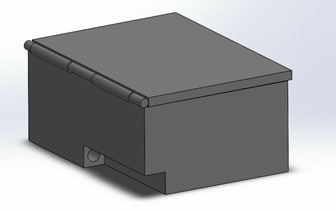
\includegraphics[width=0.45\textwidth]{casing1}
    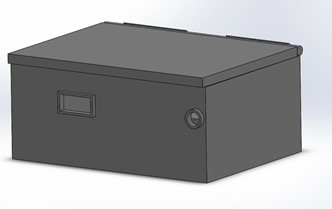
\includegraphics[width=0.45\textwidth]{casing2}
    \caption{Tracker Device Casing}
    \label{fig2}
\end{figure}

\subsection{Data Processing and Communications Module}
Data Processing Module consists of TTGO-TCall ESP32 Module. This Module has integrated SIM800L module that will act as mobile modem to connect to telecommunications mobile network. It also includes IP5306 System-on-Chip (SoC) to power up the board using battery, and controls battery charging process. This board allows for conventional communication between module via GPIO pins that are available, and providing power pins to modules such as GPS Module.

\begin{figure}[htbp]
    \centering
    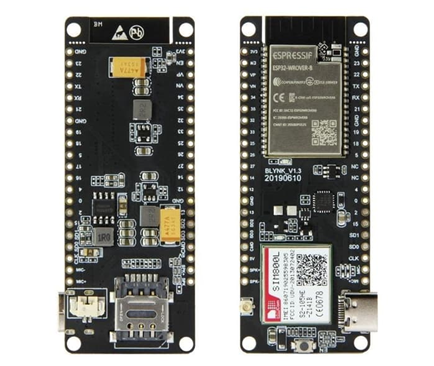
\includegraphics[width=0.45\textwidth]{gambaresp32}
    \caption{TTGO T-Call ESP32 Board with integrated SIM800L Communications Module}
    \label{fig3}
\end{figure}

\subsection{Location Sensing Module}
The functionalities of coordinate data acquisition for real time tracking and historical data collection is fulfilled by u-Blox NEO-6M Module. NEO6M module is a GNSS receiver with capabilities of receiving from US GPS satellite network. Compared to newer variants from u-Blox, notably the M8 Series receivers, the NEO-6M lacks the ability to receive data from Galileo and GLONASS satellite networks. However, as with 
the choice of SIM800L module for communication, the availability and price of the module are the key reasons on why NEO-6M is used. Communication between NEO-6M Module and ESP32 module are as follows:
\begin{itemize}
\item 'Tx' Pin on NEO-6M connects to pin 'GPIO14' of ESP32module.
\item 'Rx' Pin on NEO-6M connects to pin 'GPIO12' of ESP32module.
\end{itemize}

\subsection{Theft Detection Data Acquisition Module}
Theft detection is possible when the system meet one of the two scenarios. In the first scenario, the system will detect theft if vehicle is moving from its original position where the user initially turns on the configuration. This scneario can be fulfilled from comparing location data that has been acquired.

In the second scenario, when the vehicle engine turns on. The second scenario, however, will need additional interfacing modules to gather more information. This information is the information of the car being on or off. To get this data, the device will interface with the vehicle with On Board Diagnostics (OBDII) Port. OBDII Port are mandatory features that can be found in cars. 
While different cars have different standards for their OBDII ports, where each port can send different types of data, it is crucial for this system to be used in types of cars. Therefore, detection of engine turning on is done by monitoring for impulses in the data lines of the individual pins, where the data pins will be active only once the engine of the car is turned on.

\begin{figure}[h!]
    \centering
    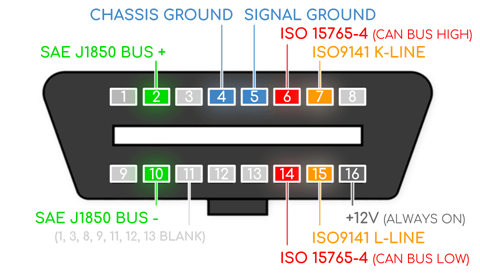
\includegraphics[width=0.45\textwidth]{obddiagram}
    \caption{Pinout Diagram of an OBDII Port}
    \label{fig4}
\end{figure}

\subsection{Backup Power Module}
The system designed will have a backup power module in the form of rechargeable Lithium-Ion Batteries. These batteries need to be able to last a certain period of heavy usage in the case of the device being unplugged from the OBDII port. 
The system uses 2 3400 mAh Panasonic NCR18650B batteries, totaling the capacity to 6800 mAh. This will be connected via a proprietary connector available in the ESP32 module, and charging will be managed by IP5306 SoC module as mentioned 
previously. 

\section{Cloud Subsystem}
Google Cloud will be the provider of the Cloud infrastructure, where multiple solutions offered by Google Cloud will work together to perform the function of transporting data from Tracker to User Interface, and vice versa.

\subsection{Google Cloud IoT Core}
Cloud IoT Core allows for securely connecting and managing IoT devices to the Google Cloud Infrastructure, and acts as the connecting bridge of these devices to other Google Cloud Solutions \cite{iotcorewebsite}. Devices connect to IoT Core via registry that is created from Google Cloud Console. This registry, when devices are connected, will be able to show a full log of input and output of the device, or the CONFIG and STATE of the device in relation to the display of the device in the log. 

\subsection{Cloud Functions}
Cloud Functions allows triggering of certain methods and functions via different solutions that are available at Google Cloud, where data from a solution can be used by another solution. One example of this is triggering a function from a change in Firestore 
Database, or triggering a change in Pub/Sub Bucket to activate certain functions \cite{cloudfunctionwebsite}. In this case. Cloud function will be used for the following:
\begin{itemize}
\item Store telemetry sent from Tracker to Firestore Database, triggered by a new publish of Data from Pub/Sub Client of the Created IoT Core Registry
\item Send configuration updates from User Interface to change the modes of the Tracker, triggered by an HTTPS request from the front end (i.e. press of a button available in the user interface)
\item Pair a device with a user account in order for it to be accessed by said account, triggered by an HTTPS request from the front end
\item Send push notifications based on change in Firestore document data, triggered by a change of data in the field of a Device Document in Firebase Firestore
\end{itemize}

\begin{figure*}[ht!]
    \centering
    \def\svgwidth{\columnwidth}
    \scalebox{1.8}{\input{figures/skematikdiagram2.pdf_tex}}
    \caption{Cloud Functions in Relation to Other Subsystems}
    \label{fig5}
\end{figure*}

\subsection{Firebase Firestore}
The database that we used for this project, divided into two main collections that are 'devices' and 'users'. The 'users' collection contain documents of all the registered users, containing email data and notification tokens to be used for receiving notifications. The name of the document uses 
the randomly generated user ID from Firebase Authentication. The 'devices' collection contain documents of all the registered and activated tracker devices, where the name of each document correspond to the name of tracker that is created when device is connected to Google IoT Core. This is to make sure that the data sent from a specific device will arrive to the correct document with the same name. The document itself contains several fields, consisting of real time longitude and latitude; owner of the tracker, which corresponds to the user ID that is generated and used by Firebase Authentication to identify a user; the fields 'Trigger' and 'ReqReal' containing values of either '0' or '1', which will be identified by the Tracker to be used to change the configuration of the device; the fields 'isConnect', 'isGPS' and 'baterai' corresponding to mobile data connection status, GPS data availability and battery level respectively; the fields 'Daya' and 'Pencurian' to identify whether the device has been plugged off from the OBDII port and to identify if the vehicle has been stolen, respectively. These data will be used from each side of the system (Tracker side and User Interface Side) by Cloud Functions and create a communication system between these two ends. Linked to the Tracker Document is a collection of historical data that will contain historical data documents. These historical data documents consist of latitude, longitude and timestamp data to differentiate themselves from each other.

\section{User Interface Subsystem}
This subsystem will be responsible for the user’s interaction, which includes account management functionalities such as creating and accessing accounts, receiving push notifications in regard to events such as theft detection and the unplugging of OBDII port, pairing trackers with an account, as well as a method in which to access data received from device to a presentable visual form. This subsystem will also allow the user to control different configurations of the device, in order to change the behavior of the device. The user interface is built as a Progressive Web App, essentially a website with a service worker to implement functions such as offline caching and notification event listening. Progressive Web Apps also allow the user to install the application as if the program 
is a native application for each respective device, currently supported in Windows 10, iOS and Android devices. 

This subsystem consists of multiple pages, each performing a different task. Login page will be used for both creating a new account and login to an existing account. Dashboard page will be the main page to access telemetry Data such as real time location, availability of mobile network and GPS data, and backup power reserve percentage. Dashboard also allows initial pairing of device to the account. History page will be used to access historical data of each paired device. All of the location data will be displayed via Google Maps and shown in relation with the current location of the user via their geolocation data. 

\subsection{Firebase Authentication}
Firebase Authentication will be used to handle account management request, such as creating an account, verifying an account and accessing an already created account. Firebase Authentication allows a simple implementation of authentication as it is in the form of a ready-to-use function that can be called from the Firebase Authentication SDK. Firebase Authentication allows multiple methods of 
account creation, such as Google Account Login or Facebook Account Login. In this system, the user can create an account with an email, then set a password and lastly will be able to verify their account via email verification. Users who are able to verify their accounts  can log in and access the Dashboard page where the user will be able to add/pair activated trackers. The figure below the design of the User Interface for register and login processes.


\subsection{Firebase Cloud Messaging}
Firebase Cloud Messaging allows the function of implementing push notifications to users, by working together with Service Worker of the Progressive Web App application, and Cloud Functions to send notifications such as a warning that the vehicle has been stolen, and a message regarding disconnect of device from OBDII port. Firebase Cloud Messaging uses tokens to trigger notifications, where the tokens will be given to a user when accessing the Dashboard page. This token will be saved in Database in the user's document section of the database. Notification will be triggered once an event happened, in this case a change on the fields of the Tracker document as mentioned previously. 

\subsection{Firebase Hosting}
Firebase Hosting will be used to serve all the resources of the application, and thus accessible via domain. One of the key advantages of using Firebase Hosting is the ability to serve securely via HTTPS and therefore communication between the user and the server is encrypted. Firebase hosting also allows deployment of different versions of the application, which is useful in a situation where a new deployment can cause problems, and a quick 'undo' action is necessary to make sure the user's experience will not be interrupted by the problematic deployment.

\subsection{Google Maps API}
Google Maps API will be used to visually display the coordinate data received from the Tracker Device. Google Maps is implemented using Maps JavaScript API that is available to be used using an API key generated on Google Cloud Console. Alongside the location data of tracker will also be the location of the user, who will use the geolocation data of the device used to access the user interface (i.e. mobile phone or desktop device). Maps API will be used to display both real time location and historical location.

\section{Results}
\subsection{Real time Tracking and Historical Data Acquisition}
Real time location data acquisition is possible through the Dashboard page. The user will first choose which Tracker Device. The chosen Tracker Device will then be selected, and the latest recorded location will be displayed in Google Maps interface, along with the location of the user accessing the application. The user will then be able to choose to turn on real time tracking to get the latest location data from a button element available in the Dashboard. Once it is selected, it will create a change in data in Firestore Database by changing the value of the 'ReqReal' field from '0' to '1', where it will be detected by a Cloud Function that is designed to detect changes in the document. 
This will then send a new configuration to the device, telling the device to turn on real time tracking, where it will provide an update at a rate of every 10 seconds, provided that GPS data is provided by the receiver.

\begin{figure}[h]
    \centering
    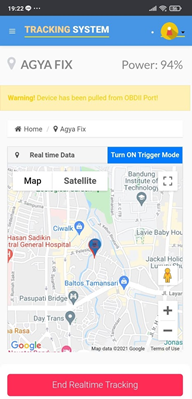
\includegraphics[width=0.2\textwidth]{realtimeon}
    \caption{Real Time Tracking Turned on in Dashboard}
    \label{fig6}
\end{figure}

The tracker device will also send historical location data automatically without prompt, providing the user with extra precaution in the case that they forgot to enable theft detection mode. Historical data can be accessed in the History page of the application.

\subsection{Theft Detection Simulation}
Theft detection is possible by turning on theft monitoring configuration, by pressing the 'Turn ON Trigger Mode' button in the dashboard Page. Turning on this future will change the 'Trigger' field from '0' to '1', and this changed will be detected by a Cloud Function, and will instruct the device to change configuration and monitor for scenarios of car theft. When theft is detected, it will send a push notification the user's device, while also displaying a message to remind the user of the situation when they access the Dashboard page. A notification will appear as shown in figure~\ref{fig7} if a theft is detected.
\begin{figure}[htbp]
    \centering
    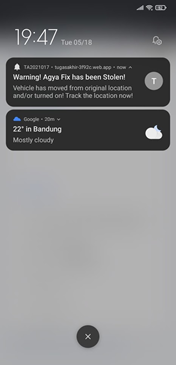
\includegraphics[width=0.15\textwidth]{notif1}
    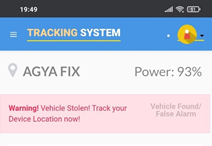
\includegraphics[width=0.25\textwidth]{notif2}
    \caption{Notification and Displayed Message when Theft is Detected}
    \label{fig7}
\end{figure}

\section{Conclusion}
A system has been designed that has been able to incorporate GPS and GPRS technology to track location of passenger cars. The system is also able to detect an act of theft through 2 predefined scenarios, which are when engine is turned on and when the vehicle has moved 50 meters from its original position. The user is able to access all of the information given by the Tracker through a user interface designed as a Progressive Web App which enables features such as push notifications to be possible in a web-based application. Communication between Tracker and User Interface is fulfilled with Google Cloud Solutions, consisting of Google IoT Core, Cloud Functions, and Firebase Firestore. Implementation is possible in passenger cars with OBDII Port, where engine-turn on data and main power is acquired. Backup power is provided by a battery pack for situations where OBDII Port is unplugged, which will also be informed to the user via push notifications. 


\section{Future Development}
This system can be enhanced further by implementing the use of 4G LTE instead of GPRS once the components are available for a more economical price point. Any technology that can be used is to use Narrowband-IoT (NB-IoT) as a means of communications once the infrastructure is available to be used for general public in Indonesia. Implementing NB-IoT will allow for less power consumption and enable the device to be powered solely by external power source, like a battery pack, and enable more reliable mobile network connection. Another development would be offering this system to motorcycles, by changing the interfacing format to the vehicle from OBDII to other means.


\bibliographystyle{IEEEtran}
\bibliography{references}

\end{document}
